\section{Theoretical Background}\label{section::theoretical_background}

\subsection{Machine Learning}
\footnote{
Note that this section is based on the lecture materials of \textit{6.036 Introduction to Machine Learning} course by MIT \cite{MITx6.036}, unless stated otherwise.}

Machine Learning is largely regarded as a subfield of AI. As its name suggests, the central concept is learning from data, through a process called training. Although the techniques are abundant, they all mostly draw their foundations from the fields of optimization and probabilistic inference. 

When describing a machine learning system, there are some foundational concepts which they all share:

\begin{itemize}
    \item \textbf{Problem Class:}
    Refers to the type of problem we are trying to solve. Some of the most common problem classes are: classification, prediction, clustering, dimensionality reduction, summarization, and translation. This will all be encompassed by the word "prediction" and the verb "predict" from this point onwards.
    \item \textbf{Assumptions:}
    It is assumed that previous data, or a subset of the data will help us to learn patterns from it that generalize to unseen data. More formally, we assume that the data we use for the learning algorithm (training data), and the rest of the data were sampled from the same probability distribution. Other assumptions that could be made depending on the problem are independence of features (characteristics of the data) and linear relationships.
    \item \textbf{Generalization:}
    As mentioned previously, the algorithm should perform well on non-training data. This is called generalization.
    \item \textbf{Learning Algorithm:}
    The learning algorithm is used to learn from data and make predictions, strongly linked to the problem class and the nature of the available training data like quantity.
    \item \textbf{Parameters:}
    Refers to the learnable part of the system. It is the piece that is used for the prediction after training, along with the architecture of the system. This vector is also called the weights of the model.
    \item \textbf{Hyperpameters:}
    These refer to adjustable values used in the learning function. Their tuning to perform better is highly coupled with the training data and the problem class. This process is usually called hyperparameter tuning.
    \item \textbf{Loss Function:}
    A mathematical function that quantifies the difference between model predictions and actual target values. It guides the training process by providing a measure to minimize.
    
    \item \textbf{Model:}
    Refers to the mathematical model comprising the architecture, and the parameters.
    
    \item \textbf{Evaluation Function:}
    Similar to the loss function, it receives the output of the model for a subset of data points (non-training data) and the target values, outputting a number signifying the distance between them. It is used to assess the performance of the model on unseen data. Some of the most common evaluation functions are the F1-score and the BLEU score, commonly used in binary classification tasks \cite{lipton2014thresholding} and translations \cite{ghassemiazghandi2024evaluation} respectively.

    The F1-score  is based on precision and recall, which are defined as follows \cite{lipton2014thresholding}:

    \begin{equation}
    \text{Precision} = \frac{\text{True Positives (TP)}}{\text{True Positives (TP)} + \text{False Positives (FP)}}
    \end{equation}

    \begin{equation}
    \text{Recall} = \frac{\text{True Positives (TP)}}{\text{True Positives (TP)} + \text{False Negatives (FN)}}
    \end{equation}

    The F1-score is given by:

    \begin{equation}
    F_1 = 2 \times \frac{\text{Precision} \times \text{Recall}}{\text{Precision} + \text{Recall}}
    \end{equation}

    The F1-score is useful because it penalizes imbalances between precision and recall, ensuring that a model is not rewarded for excelling in one while failing in the other. For example, a classifier that labels all instances as positive may achieve high recall but low precision, making it ineffective. The F1-score prevents such misleading results by considering both metrics together.

    \item \textbf{Overfitting:}
    This is the opposite of generalizing. When a model overfits, it means it performs well on the training data, but not on unseen data. It is conventionally said that the model memorized the training data.

    \item \textbf{Underfitting:}
    The model does not perform well on the training data or unseen data. It is usually assumed that the model either needs further training, or the nature of the data is more complex than what the model can capture (e.g., using a linear separator to classify non-linearly separable data).
    
\end{itemize}
    Approaches in the field for training models can usually be categorized into supervised learning, unsupervised learning, semi-supervised learning and reinforcement learning. Supervised learning is the method used in this work and its core is using the labels of the data in the training process to continuously reduce the output of the loss function.
    
    One of the most common models in machine learning is the neural network. Because of their high number of parameters, they provide great flexibility for complex tasks, a characteristic that also makes them usually require greater volumes of data than other classical machine learning algorithms such as Naive Bayes \cite{osisanwo2017supervised}, a statistical model based on the Bayes Theorem \cite{webb2010naive},

\subsection{Deep Learning}
\footnote{
Note that this section is based on the lecture materials of \textit{6.036 Introduction to Machine Learning} course by MIT \cite{MITx6.036}, unless stated otherwise.}

As explained in \textit{Deep Learning} \cite{goodfellow2016deep}, modern deep learning is defined as a class of machine learning algorithms that construct complex architectures by composing simpler structures. However, most contemporary interpretations focus on neural networks \cite{goodfellow2016deep}.
     
    Neural networks, because of their aforementioned properties, are suitable for learning patterns from complex high-dimensional data. Before starting with them, some machine learning concepts need to be defined more formally:

    \textbf{Data point}

    A mapping from data point to vector is needed for neural networks since most operations involve vector products. There are several ways to do this, but to illustrate this concept, and the next ones, a data point x with D features will be mapped to ${\mathbb{R} ^ {D, 1}}$ (i.e. a column vector with D dimensions).

    \textbf{Loss Function}

A loss function measures the discrepancy between the predicted output and the true label. Formally, a loss function for one data point is defined as:

\begin{equation}
    \mathcal{L}: \mathbb{R}^{D, 1} \times \mathbb{R}^{D, 1} \rightarrow \mathbb{R}
\end{equation}

where \( D \) is the dimension of the data and the labels.

One of the most commonly used loss functions for classification tasks is the cross-entropy loss, which measures the difference between the predicted probabilities for each class and the actual class labels. Cross-entropy is especially useful in tasks where the model outputs a probability distribution over multiple classes.

In the multiclass setting, the cross-entropy loss is defined as:

\begin{equation}
    L_{\text{CE}} = - \sum_{c=1}^{C} y_c \log(p_c)
\end{equation}

where:
\begin{itemize}
    \item \( C \) is the total number of classes,
    \item \( y_c \) is a binary indicator (0 or 1) that denotes whether class \( c \) is the true label for the input, and
    \item \( p_c \) is the predicted probability that the input belongs to class \( c \).
\end{itemize}

For binary classification, where the task is to distinguish between two classes (e.g., positive and negative), the cross-entropy loss simplifies to:
\begin{equation}
L_{\text{CE}}(p, y) = - \left( y \log(p) + (1 - y) \log(1 - p) \right)
\end{equation}


where:
\begin{itemize}
    \item \( y \in \{0, 1\} \) is the actual label (0 for the negative class and 1 for the positive class),
    \item \( p \) is the predicted probability for the positive class.
\end{itemize}

    
    \textbf{Parameters}
    
    They are learned from data by the learning algorithm and are the main characters in making predictions after training. From this point on, every time the parameters are mentioned, it refers to a vector $\theta \in \mathbb{R} ^ {D, 1}$, with D being the dimension of the data point.
    
    \textbf{Gradient Descent}

    An optimization algorithm, in which the gradient of the loss function is used to update the parameters to minimize the loss (output of the loss function). It can be pictured as going in the opposite direction of the gradient (the steepest descent). More formally, having  $\nabla_\theta \mathcal{L}$, the update of the parameters can be thought of as 
    \begin{equation}
        \theta \coloneq \theta - \eta \nabla_\theta \mathcal{L}
    \end{equation}
    with \(\eta\) being a hyperparameter of the learning algorithm called the learning rate, which determines how big the update of $\theta$ will be.


    \subsubsection{Neural Networks}

    Neural Networks or Artificial Neural Networks are a machine learning model, whose architecture is inspired by the human brain. For brevity, the following descriptions in this subchapter will pertain to a simple type of neural networks called a Feed Forward Neural Network.
    
    The architecture looks like the figure \ref{fig:ffnn} and the figure \ref{fig:simulation_brain} is a computer simulation of the neural network structure in the brain.


\noindent
% \begin{minipage}[c]{0.5\textwidth}
% \centering
\begin{figure}
\centering
\begin{tikzpicture}[scale=1, x=2.2cm,y=1.4cm ]
  \message{^^JNeural network without text}
  \readlist\Nnod{4,5,5,5,3} % array of number of nodes per layer
  
  \message{^^J  Layer}
  \foreachitem \N \in \Nnod{ % loop over layers
    \def\lay{\Ncnt} % alias of index of current layer
    \pgfmathsetmacro\prev{int(\Ncnt-1)} % number of previous layer
    \message{\lay,}
    \foreach \i [evaluate={\y=\N/2-\i; \x=\lay; \n=\nstyle;}] in {1,...,\N}{ % loop over nodes
      
      % NODES
      \node[node \n] (N\lay-\i) at (\x,\y) {};
      
      % CONNECTIONS
      \ifnum\lay>1 % connect to previous layer
        \foreach \j in {1,...,\Nnod[\prev]}{ % loop over nodes in previous layer
          \draw[connect,white,line width=1.2] (N\prev-\j) -- (N\lay-\i);
          \draw[connect] (N\prev-\j) -- (N\lay-\i);
          %\draw[connect] (N\prev-\j.0) -- (N\lay-\i.180); % connect to left
        }
      \fi % else: nothing to connect first layer
      
    }
  }
  
  % LABELS
  \node[above=0.5,align=center,mygreen!60!black] at (N1-1.90) {input\\[-0.2em]layer};
  \node[above=0.5,align=center,myblue!60!black] at (N3-1.90) {hidden layer};
  \node[above=0.7,align=center,myred!60!black] at (N\Nnodlen-1.90) {output\\[-0.2em]layer};
  
\end{tikzpicture}
% \captionof{figure}{Simple Neural Network \cite{mit_neural_networks}} 
\caption{Feed Forward Neural Network \cite{tikz_neural_networks}}
\label{fig:ffnn}
\end{figure}

\begin{figure}
    \centering
    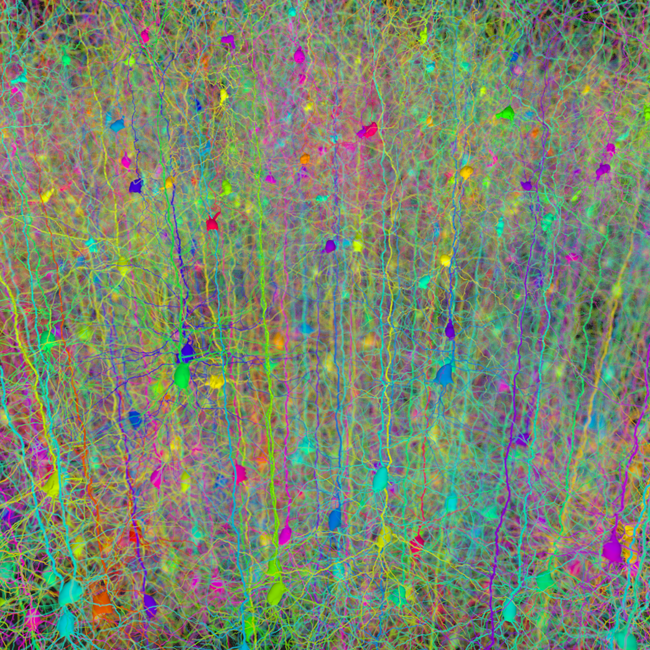
\includegraphics[width=0.5\textwidth]{neural_networks_brain.png}
    \caption{Brain Neural Network Simulation}
    \label{fig:simulation_brain}
\end{figure}


\bigskip

Both pictures show neurons or nodes propagating information.

The central component of a neural network is the artificial neural neuron (See Figure \ref{fig:ANN}), whose inspiration in the human brain comes from the nerve cells (See Figure \ref{fig:HN}).

\begin{figure}
    \centering
     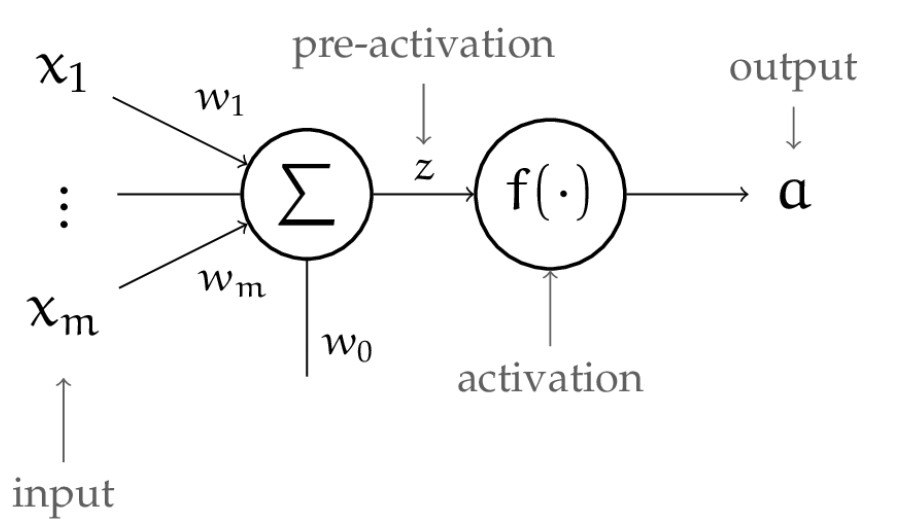
\includegraphics[scale=0.4]{neural_network_mit.png}
    \caption{Artificial Neural Neuron \cite{mit_neural_networks}}
    \label{fig:ANN}
\end{figure}

\begin{figure}
    \centering
    % Second image (your external PNG)
    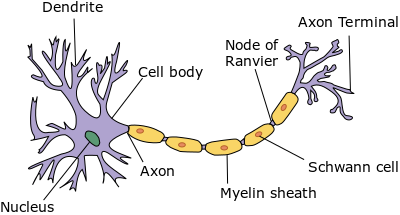
\includegraphics[scale=0.25]{Neuron.png}
    \caption{Human Neuron \cite{seer_neurons}}
    \label{fig:HN}
\end{figure}
The neuron is the processing unit in the architecture. One of the earliest models of such a unit is the perceptron, introduced by Frank Rosenblatt \cite{block1962perceptron}, which performs a weighted sum of inputs. It is a linear classifier for binary classification that computes the sum:

\begin{equation}
z = \sum w_i x_i + b
\end{equation}

where \( w_i \) are the weights, \( x_i \) are the inputs, and \( b \) is the bias term, which prevents the decision boundary from being constrained to pass through the origin. The output is then determined by the function:

\begin{equation}
f(z) =
\begin{cases} 
1, & \text{if } z \geq 0 \\
0, & \text{if } z < 0
\end{cases}
\end{equation}


The neurons are arranged in layers. Each layer uses the previous layer's outputs for its calculations and then forwards its outputs to the next layer.

Neurons are arranged in layers. Each layer uses the previous layer's outputs for its calculations and then forwards its outputs to the next layer.  For a given layer \( l \), the computation follows:

\begin{equation}
    z^{(l)} = W^{(l)} a^{(l-1)} + b^{(l)}
\end{equation}

\begin{equation}
    a^{(l)} = \sigma(z^{(l)})
\end{equation}

where \( W^{(l)} \) is the weight matrix, \( a^{(l-1)} \) represents the outputs (activations) from the previous layer, \( b^{(l)} \) is the bias vector, and \( \sigma(\cdot) \) is the activation function. 

There are typically three kinds of layers:

\textbf{Input Layer}

The input layer is a symbolic name since it refers to the input data points, with each node in the layer usually representing a feature of the data points. There is just one input layer.

\textbf{Hidden Layer} 

This is where the bulk of operations take place. They usually compose the majority of the layers.

\textbf{Output Layer}

Aggregates the inputs of the last hidden layer making sense of the data to get an output, which should be interpretable as a result of the specific task (regression, classification).


For complex tasks usually many hidden layers are required in neural networks, which define and give the name to the field of deep learning.

\subsubsection{Training}

The following explanation refers specifically to supervised training.

Training a model can be viewed as a minimization problem where the goal is to minimize this loss function over time. This process of minimization is what enables the model to improve its predictions.

There are typically two stages in a training loop: forward pass and backpropagation.

\textbf{Forward Pass}

The forward pass is the process where input data propagates through the neural network layer by layer until it reaches the output. Each neuron in a layer takes inputs from the previous layer, applies weights and biases, and then passes the result through an activation function.  

In training, this step generates predictions based on the current model parameters. The key steps are:  
\begin{itemize}
    \item The input layer receives raw data (e.g., images, text, or numerical values).  
    \item The data is transformed as it moves through hidden layers, where each layer extracts increasingly abstract features.  
    \item The final layer produces an output, which could be a probability distribution (for classification) or a numerical value (for regression).  
\end{itemize}  

After the forward pass, the model's predicted output is compared to the true label or value using a \textbf{loss function}, which quantifies the error. The computed loss serves as feedback for weight updates through backpropagation.  

\bigskip  

\textbf{Backpropagation} 

Backpropagation is an optimization algorithm that updates the weights of the neural network using gradient descent. It computes the gradient of the loss function with respect to each weight in the network, starting from the output layer and propagating backward through the network. This process relies on the chain rule of calculus.  

The key steps in backpropagation are as follows:

\begin{enumerate}
    \item \textbf{Compute the loss:}
    The difference between the predicted output and the true value is measured using a loss function \( L \).  
    \item \textbf{Calculate the gradient at the output layer:}  
    \begin{equation}
        \frac{\partial L}{\partial a^{(L)}}
    \end{equation}
    This represents how much the loss changes concerning the output of the last layer.
    \item \textbf{Propagate the gradients backward:}  
    Using the chain rule, the gradient of the loss with respect to the weighted input of the last layer is computed as:
    \begin{equation}
        \frac{\partial L}{\partial z^{(L)}} = \frac{\partial L}{\partial a^{(L)}} \odot \sigma'(z^{(L)})
    \end{equation}
    where \( \sigma'(z^{(L)}) \) is the derivative of the activation function.  

    The weight and bias gradients for layer \( L \) are given by:
    \begin{equation}
        \frac{\partial L}{\partial W^{(L)}} = \frac{\partial L}{\partial z^{(L)}} a^{(L-1)T}
    \end{equation}
    \begin{equation}
        \frac{\partial L}{\partial b^{(L)}} = \frac{\partial L}{\partial z^{(L)}}
    \end{equation}

    These gradients are recursively propagated backward through each layer.
    \item \textbf{Update the weights using gradient descent:}  
    \begin{equation}
        W^{(l)} = W^{(l)} - \eta \frac{\partial L}{\partial W^{(l)}}
    \end{equation}
    \begin{equation}
        b^{(l)} = b^{(l)} - \eta \frac{\partial L}{\partial b^{(l)}}
    \end{equation}
    where \( \eta \) is the learning rate.
\end{enumerate}

This process of forward pass, loss computation, backpropagation, and weight update is repeated iteratively until the network converges to a set of parameters that minimize the loss function or after a set number of iterations.

\subsubsection{Natural Language Processing}

\begin{definition}
    Natural language processing (NLP) is the use of human languages, such as
English or French, by a computer \cite[p.461]{goodfellow2016deep}. 
\end{definition}

The field involves analyzing natural language and sometimes predicting from it \cite{goodfellow2016deep} and is largely viewed as a subfield of machine learning since the most common approach used in modern NLP is deep learning \cite[Preface, p. xi]{zhang2021natural}.

\subsection{Large Language Models}
This section is based on the book Deep Learning by Ian Goodfellow \cite{goodfellow2016deep} unless stated otherwise.

Refer to deep learning models focusing on NLP, mainly on text. They have a large number of parameters, which gives them their name and are currently the state-of-the-art solution in the field of Natural Language Processing. They are the current answer to the high complexity posed by natural language, such as cultural references, syntax, semantics, and nuance.

The current most used architecture is called the Transformer Architecture and it aims to tackle the lack of parallelization possible in the previous models, sequential in essence \cite{vaswani2017attention}. It reduces training time significantly, in a task like translation between languages, from several days \cite{bahdanau2014neural} to as little as twelve hours.

\subsubsection{Embeddings}

Since the operations involved in training and prediction of neural networks are only defined with numerical data, a two-way representation between natural language and tensors of numbers is needed. One type of such numerical representation is called embeddings.

\begin{definition}
    Embeddings are vector representations of natural language usually learned by deep learning models, that encode semantic knowledge about words and concepts \cite{goodfellow2016deep}.
\end{definition}
A token is a discrete unit of text, such as a word, a sub-word or even a character.

The first step to process input text is breaking it up into tokens, which in modern approaches are usually sub-words, averaging about 4 characters in length in the English language in the SOTA model family of GPT are about 4 characters \cite{OpenAITokens}.

These tokens are then usually mapped to IDs through the vocabulary, which is a look-up table mapping text tokens to numeric IDs.

Finally, additional contextual information is embedded into the IDS during training of most modern models in NLP. They are updated based on surrounding tokens and relative position. For example the token "how" could have different embeddings in the sentences "How are you?" and "That is how you do it".


\subsection{Transformer Architecture}


The main new breakthrough coming with the transformer architecture is the ability to process tokens in parallel while also keeping the dependencies of the ones far apart in the text input. This provides both a significant speed up in training as well as an increase in performance in certain tasks such as machine translation from English to German \cite{vaswani2017attention}.

\subsection{Transfer Learning}

Refers to leveraging training in one task to train a machine learning model in another, usually related task. \cite{torrey2010transfer}. 

A special kind of transfer learning, called cross-lingual transfer, revolves around leveraging training in one language to improve the results of training in another language \cite{cross_lingual_transfer}.

\subsection{Continual Pre-training of Large Language Models}
Refers to the addition of new data as knowledge base to an already trained large language model without merging the old dataset and the new one to start the training from scratch \cite{gupta2023continual}.

It consists mainly of the careful selection of a learning rate to minimize the loss on new data while maintaining the loss on the original data. This is a key factor in the process since the distribution shift that further training introduces can lead to a decrease in performance in previous (original) data. Research indicates that the right parameters might make continual pre-training better performing than training from scratch on the whole data \cite{gupta2023continual}.


\subsection{Semantic Web}

An initiative to make web content machine-readable by standardizing it \cite{pellegrini2006semantic}.

Resource Description Framework (RDF) is one of the most popular frameworks for standardizing and representing web content. It was first introduced and encouraged by the World Wide Web Consortium (Organization developing the standards of the Web) in 1999 \cite{dataeuropa_rdf_sparql}, proposing a graph structure linking web contents making the relationships between contents machine-readable, with SPARQL being the standard query language for this format.



